\documentclass[border=4pt]{standalone}

\usepackage{tikz}

\definecolor{otblue}{HTML}{0072B2}
\definecolor{otorange}{HTML}{E69F00}
\definecolor{otteal}{HTML}{009E73}
\definecolor{otpurple}{HTML}{CC79A7}
\definecolor{otgray}{HTML}{5A5A5A}

\begin{document}
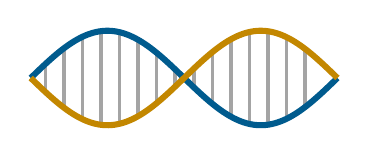
\begin{tikzpicture}[line width=0.9pt]
  \foreach \t in {0.3,0.68,...,5.9}{\pgfmathsetmacro{\y}{0.6*sin(\t r)}\draw[otgray!55, line width=1.3pt] (\t*0.62,\y) -- (\t*0.62,-\y);}
  \draw[otblue!80!black, line width=2.2pt] plot[smooth, domain=0:6.283, samples=60] ({\x*0.62},{0.6*sin(\x r)});
  \draw[otorange!85!black, line width=2.2pt] plot[smooth, domain=0:6.283, samples=60] ({\x*0.62},{-0.6*sin(\x r)});
\end{tikzpicture}
\end{document}
